\chapter{Datos} \label{a.datos}

\section{Esquema relacional de la base de datos \textit{JHipster}}


\begin{figure}[h!]
   
    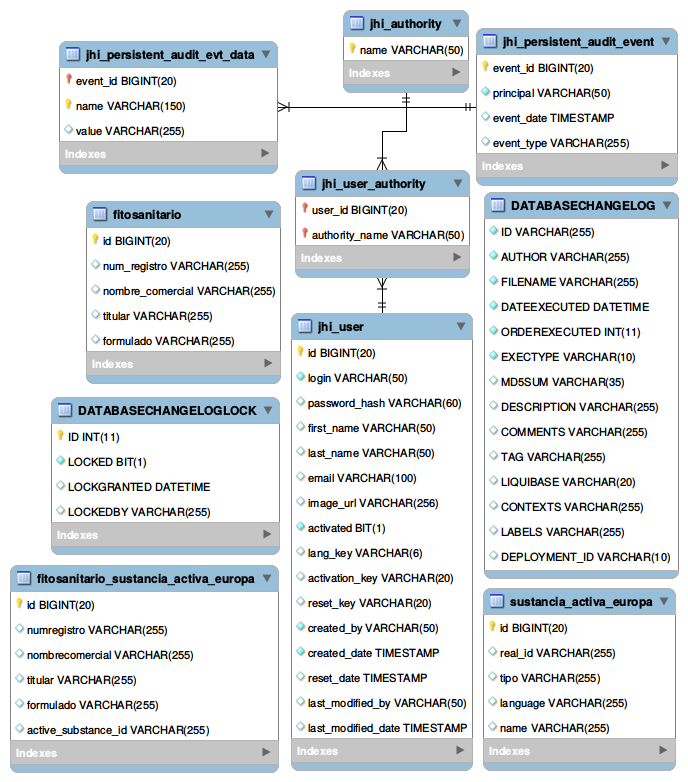
\includegraphics[width=\textwidth]{Imagenes/relational}
    \caption{Esquema relacional de la base de datos de \textit{JHipster}}
    \label{fig:relacionalmysql}
\end{figure}


\begin{landscape}
\section{Esquema de datos en la base de datos MySQL} \label{a.datos.modelo}
\begin{figure}[h!]
    
    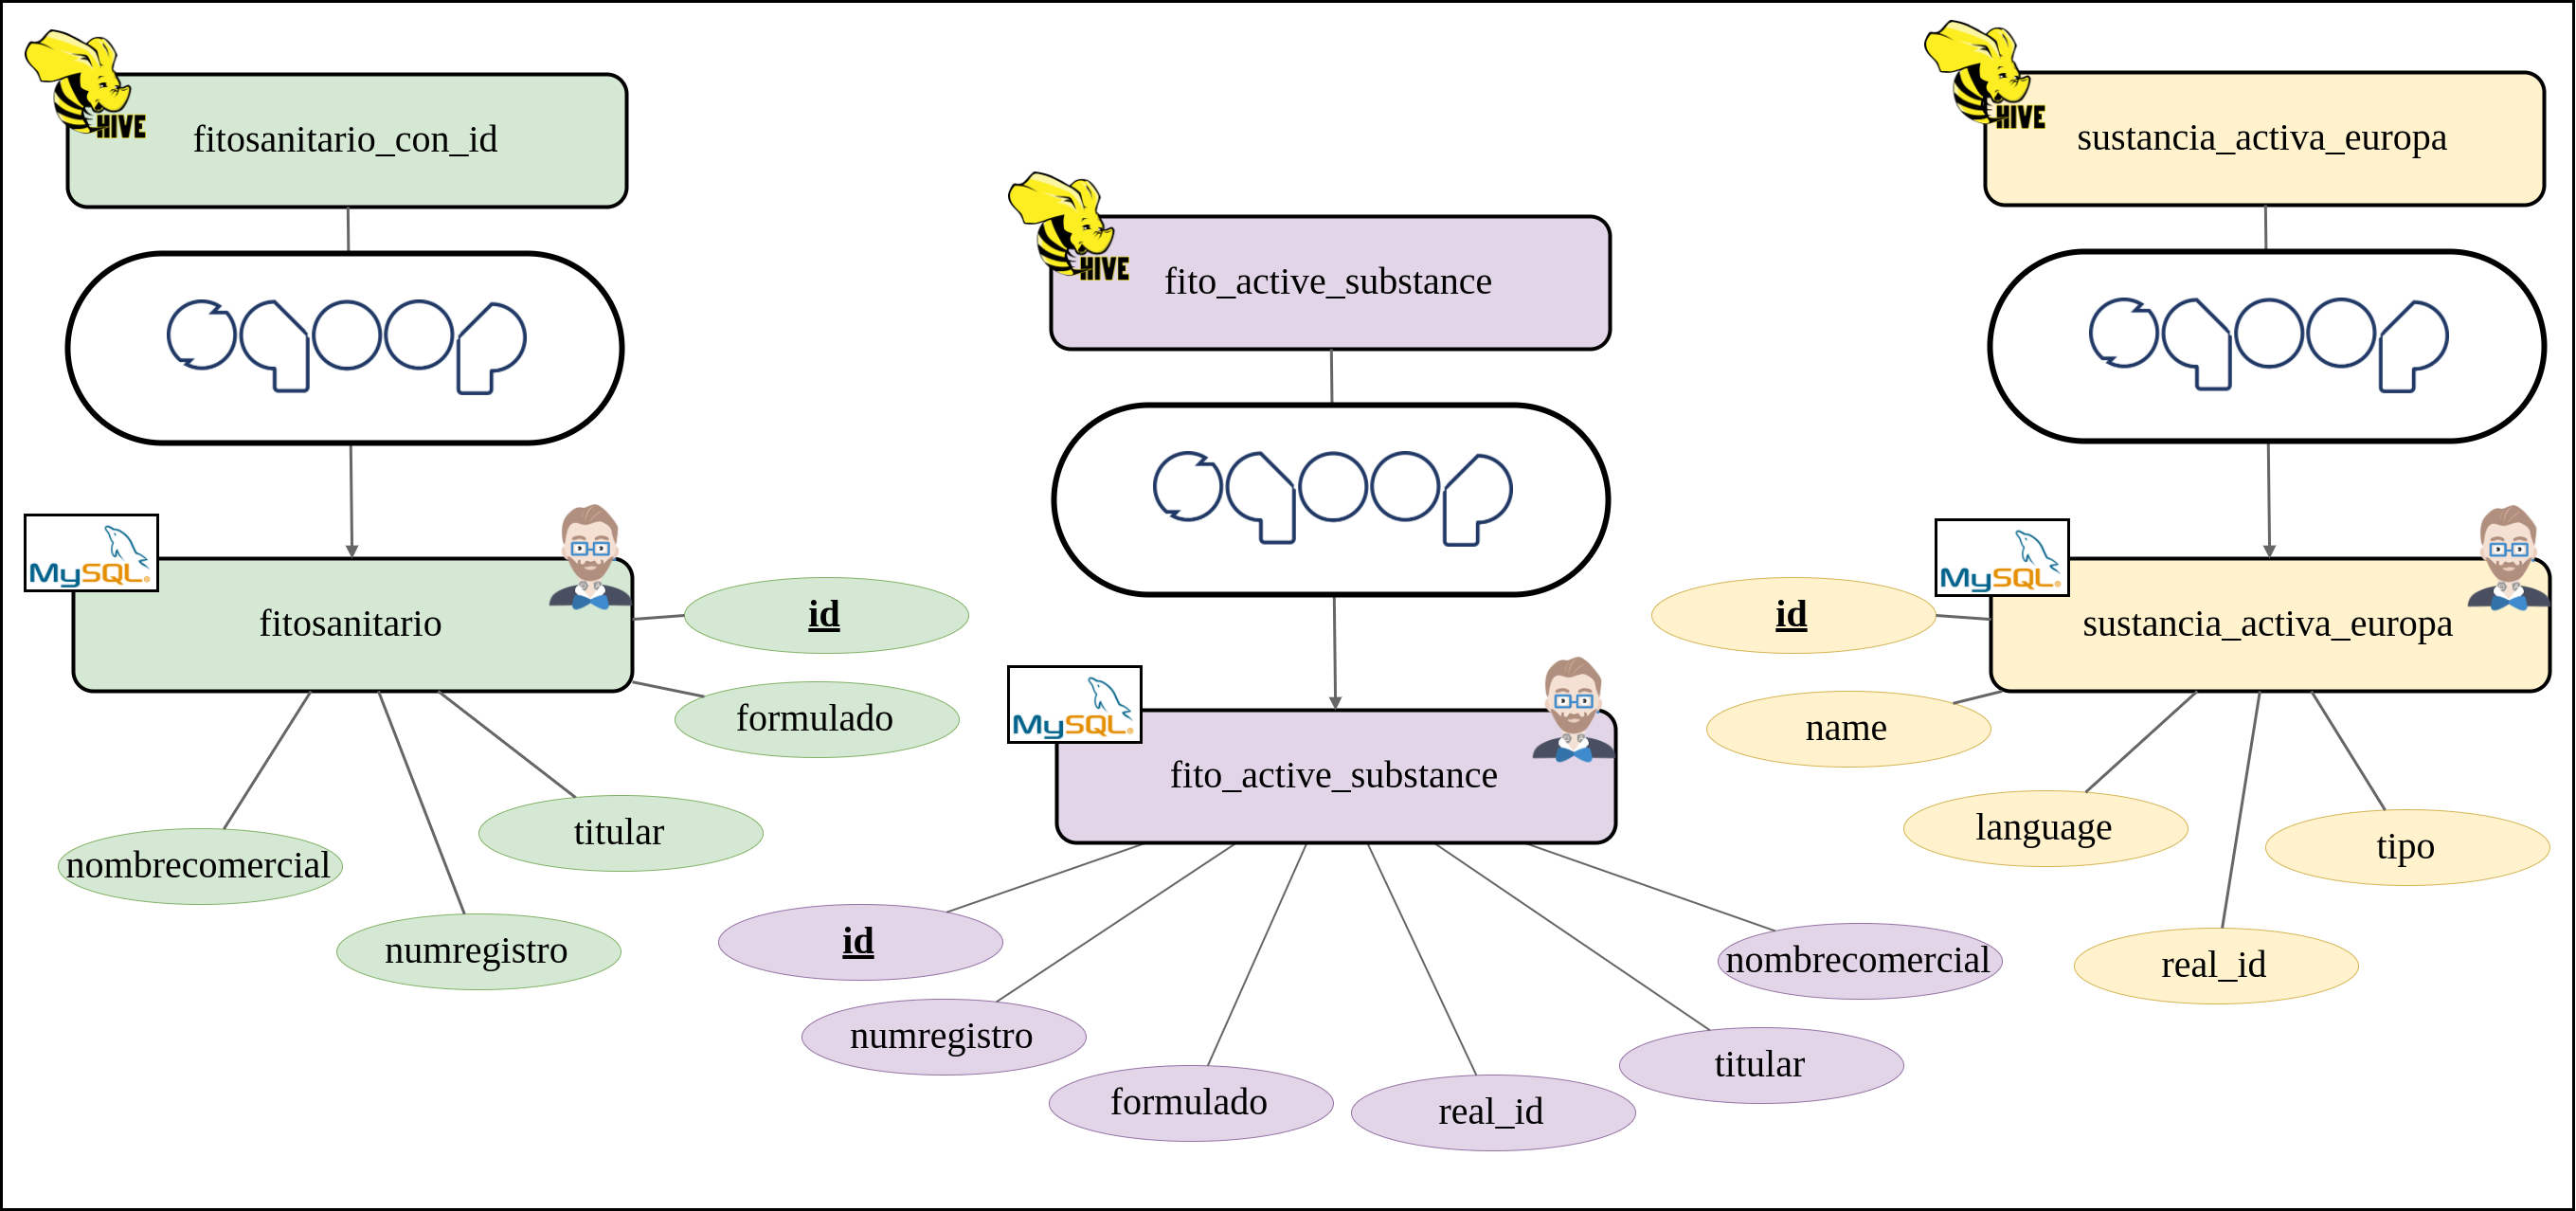
\includegraphics[width=1.5\textwidth]{Imagenes/datosmysql}
    \caption{Esquema de datos importados en \textit{MySQL} y \textit{JHipster}}
    \label{fig:datosmysql}
\end{figure}

\end{landscape}
